% !TeX spellcheck = fr_FR
\documentclass[letterpaper, 12pt]{article}
\usepackage[top = 1.6cm, left = 2cm, right = 2cm ]{geometry}
\usepackage[pdftex]{graphicx}
\usepackage{soulutf8}
\usepackage{amsmath}
\usepackage{tikz}
\usepackage[utf8]{inputenc}
\usepackage{longtable}
\usepackage[T1]{fontenc}
\usepackage{epigraph}
\usepackage{fancyhdr}
\usepackage{float}
\usepackage{subfig}
\usepackage{xcolor}
\usepackage{eurosym}
\usepackage{calc}
\usepackage{multirow} 
%
%
%%%%% Custom commands
%
%
\def\changemargin#1#2{\list{}{\rightmargin#2\leftmargin#1}\item[]}
\let\endchangemargin=\endlist 
%
\newcommand{\newlinealinea}{
~\\ \hspace*{0.5cm}}
%
\newcommand{\alinea}{
\hspace*{0.5cm}}
%
\newcommand{\alinealong}{
\hspace*{1.1cm}}
%
\newcommand{\alignparagraph}{
\hspace*{0.6cm}}
%
\newcommand{\red}[1]{
	\textcolor{red}{#1}}
%
\newcommand{\green}[1]{
	\textcolor{green}{#1}}
%
\newcommand{\point}{$\bullet\ $}
%
\makeatletter
	\newcommand*{\whiten}[1]{\llap{\textcolor{white}{{\the\SOUL@token}}\hspace{#1pt}}}
	\newcommand{\myul}[1]{
		\underline{\smash{#1}}
	}
\makeatother
%
\setlength{\fboxsep}{2pt}
%
\DeclareMathOperator*{\argmax}{\arg\!\max}
%
%
%%%%% Custom text
%
%
\makeatletter
\@addtoreset{section}{part}
\makeatother  
\renewcommand\partname{Partie} 
%
\renewcommand*\sfdefault{phv}
\renewcommand*\rmdefault{ppl}
%
\renewcommand\epigraphflush{flushright}
\renewcommand\epigraphsize{\normalsize}
\setlength\epigraphwidth{0.7\textwidth}
%
\definecolor{titlepagecolor}{cmyk}{0.24,0.92,0.78,0.25}
\definecolor{red}{cmyk}{0, 0.91, 0.91, 0.20}
%
\DeclareFixedFont{\titlefont}{T1}{phv}{\seriesdefault}{n}{0.375in}
%
%
%%%%% Header
%
%
\pagestyle{fancy}
\lhead{Anthony Rouneau}
\rhead{MAB2 Sciences Informatiques}
\cfoot{\thepage}
%
%
%%%%% Title page. The following code is borrowed from: 
%%%%%       http://tex.stackexchange.com/a/86310/10898
%
%
\newcommand\titlepagedecoration{%
\begin{tikzpicture}[remember picture,overlay,shorten >= -10pt]

\coordinate (aux1) at ([yshift=-70pt]current page.north east);
\coordinate (aux2) at ([yshift=-460pt]current page.north east);
\coordinate (aux3) at ([xshift=-6cm]current page.north east);
\coordinate (aux4) at ([yshift=-150pt]current page.north east);

\begin{scope}[titlepagecolor!40,line width=12pt,rounded corners=12pt]
\draw
  (aux1) -- coordinate (a)
  ++(225:5) --
  ++(-45:5.1) coordinate (b);
\draw[shorten <= -10pt]
  (aux3) --
  (a) --
  (aux1);
\draw[opacity=0.6,titlepagecolor,shorten <= -10pt]
  (b) --
  ++(225:2.2) --
  ++(-45:2.2);
\end{scope}
\draw[titlepagecolor,line width=8pt,rounded corners=8pt,shorten <= -10pt]
  (aux4) --
  ++(225:0.8) --
  ++(-45:0.8);
\begin{scope}[titlepagecolor!70,line width=6pt,rounded corners=8pt]
\draw[shorten <= -10pt]
  (aux2) --
  ++(225:3) coordinate[pos=0.45] (c) --
  ++(-45:3.1);
\draw
  (aux2) --
  (c) --
  ++(135:2.5) --
  ++(45:2.5) --
  ++(-45:2.5) coordinate[pos=0.3] (d);   
\draw 
  (d) -- +(45:1);
\end{scope}
\end{tikzpicture}%
}
%
\begin{document}
	\begin{titlepage}
	%
	\noindent
	%
	\newgeometry{bottom = 2cm, top = 2.5cm}
	\begin{center}
		
\includegraphics[scale=1.2]{Images/UMONS}\\
			\vspace*{0.3cm}
		
\includegraphics[scale=0.23]{Images/FS_Logo}\\
			\vspace*{2.5cm}
		%
		\titlefont Statistical Pattern Recognition\\~\\ {\huge Résumé} \par
		%
	\end{center}
	\vspace*{3cm}
	\hfill
	%
	\begin{minipage}{0.18\linewidth}
		\begin{flushright}
			\rule{0.5pt}{75pt}
		\end{flushright}
	\end{minipage}
	%
	\begin{minipage}{0.8\linewidth}
		\begin{flushleft}
			\textsf{\textbf{Résumé réalisé par:}} Anthony Rouneau\\
			\textsf{\textbf{Section:}} 2$^{\text{\`eme}}$ Bloc Master en 
				Sciences Informatiques\\
			\textsf{\textbf{Images:}} Proviennent du cours de M. Gosselin.\\
		\end{flushleft}
	\end{minipage}
	%
	\vspace*{\fill}                                                             
	%
	\begin{center}
		Faculté des Sciences $\bullet$ Université de Mons $\bullet$ 
		Place du Parc 20 $\bullet$ B-7000 Mons
	\end{center}
	%
	\titlepagedecoration
	%
\end{titlepage}
%
%
%%%% Tables des matières
%
%
\newgeometry{top = 3cm, left = 2cm, right = 2cm, bottom=2.5cm}
%
\tableofcontents
%
\newpage
%
%
\part{Introduction}
	\section{Bases}
		\subsection{Principes}
			\begin{itemize}
				\setlength\itemsep{0cm}
				\item \red{Analyse statistique} -- Se fait lorsque peu de théorie est disponible sur le sujet, mais que beaucoup de 
					données le sont.
				\item \red{Pattern (modèle)} -- Objet, procédé ou évènement descriptible par un ensemble d'attributs
					venant d'observations ou de mesures.
				\item \red{Reconnaissance} -- Assigner une catégorie à un modèle donné, en choisissant dans un ensemble de possibilités.
			\end{itemize}
			%
		%
		\subsection{Définitions}
			\alinea Ci-dessous se trouvent les définitions de bases pour parler de reconnaissance statistique de modèles.
			\begin{itemize}
				\setlength\itemsep{0cm}
				\item \red{Base de données} -- Banque contenant un \hl{grand nombre} de données \hl{pouvant être libellées} d'une classe.
				\item \red{Extraction d'attributs} -- \hl{Identification et sélection} d'un ensemble fini d'attributs qui 
					\hl{représentent de manière fidèle et robuste} les objets à classifier. \hl{\'Etape cruciale} pour la qualité
					du modèle. On peut distinguer deux étapes : \hl{l'extraction et la sélection des attributs.}
					Quelques contraintes peuvent s'appliquer à cette étape comme garder la compréhensibilité des attributs utilisés
					dans le modèle ou encore n'utiliser que des attributs faible en coût d'acquisition (dépend des capteurs).
				\item \red{Classification} -- \hl{Créer et entraîner} un modèle statistique grâce aux données disponibles afin de pouvoir
					\hl{classer de nouvelles données} ne se trouvant pas dans les données d'entraînement.
					Le but final étant d'obtenir une \hl{fonction de discrimination} permettant de libeller de nouvelles données.
				\item \red{Validation} -- \hl{Vérifier la qualité} du modèle en utilisant des données \hl{"gound-truth"}. De telles 
					données sont récoltées dans des conditions réelles, et ne sont pas des données "de laboratoire".
			\end{itemize}
		%
		\subsection{Validation}
			\alinea Afin de valider le modèle statistique, plusieurs notions sont nécessaires.
			%
			\subsubsection{Probabilité d'erreur (PoE)}
				\alinea Cette mesure est calculée par l'intégrale du "coût de classification erronée" ($\delta$).
					\begin{center}
						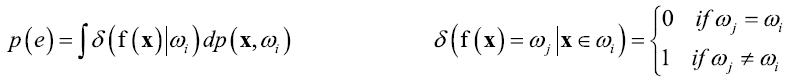
\includegraphics[width=5in]{Images/PoE} 
					\end{center}
				Cependant, elle est généralement calculée \hl{de manière discrète} en comptant sur un ensemble fini de données
				(Attention au risque empirique en faisant cela), il suffit de \hl{compter le nombre d'instances incorrectement 
				libellées}.
					\begin{center}
						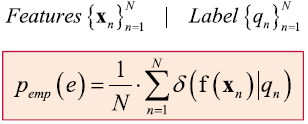
\includegraphics[width=1.75in]{Images/PoE2} 
					\end{center}
				%
				La \hl{probabilité d'erreur d'un modèle aléatoire} est de $\frac{m-1}{m}$, $m$ étant le nombre de classes considérées.
				%
			%
			\subsubsection{Risque empirique}
				\alinea Risque dépendant de la \hl{qualité des données}. Le risque augmente lorsque des données non représentatives 
					se trouve dans la base de données, ou encore lorsque des données de laboratoires se trouvent dans cette dernière.
					Réduire ce risque consiste à supprimer les "outliers" (le bruit) des données et à collecter des données de qualité
					et représentatives (ground-truth).\\
				%
				~\\
				%
				\alinea Lors de l'entraînement, prendre un \hl{modèle à haute capacité permet de réduire le risque empirique},
					mais cela pourrait augmenter le risque structurel. La validation vise à trouver un bon compromis entre un 
					risque empirique faible et une petite capacité pour le modèle.
				%
				%
			%
			\subsubsection{Risque structurel}
				\alinea Risque venant d'\hl{incertitudes et de suppositions théoriques}. Ce risque se voit augmenter lorsque 
					le \hl{modèle} statistique est \hl{trop simple (under-fitting) ou trop complexe (over-fitting)} 
					(capacité du modèle) pour le problème ciblé, ou encore lorsque le nombre de dimensions est réduit. Réduire 
					ce risque consiste à optimiser le modèle et à éviter les suppositions.
				%
				\begin{center}
					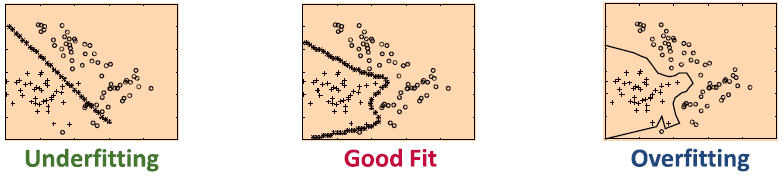
\includegraphics[width=3.66in]{Images/structural} 
				\end{center}
				%
			%
			\subsubsection{Méthodes de validation}
				\begin{itemize}
					\setlength\itemsep{0cm}
					\item \red{Resubstitution} -- Les même données sont utilisées pour entraîner et valider. \hl{Le taux d'erreur est
						alors sous-estimé}.
					\item \red{Leave-One-Out} -- Tour à tour, \hl{une donnée est écartée} pour servir de donnée de validation pendant
						que le reste des données est utilisé pour entraîner le modèle. \hl{Calculs importants} !
					\item \red{K-fold} -- On divise en \hl{K ensembles les données}, et chacun à leur tour, les ensembles sont utilisés
						comme données de validation pendant que le reste entraîne le modèle. Selon la valeur de K, \hl{beaucoup de calculs}.
					\item \red{Hold-out} -- Diviser en deux ensembles de tailles quelconques la base de données, et en utiliser un pour
						entraîner et l'autre pour valider. Attention au risque empirique qui peut augmenter car on diminue le nombre 
						de données d'entraînement.
				\end{itemize}
				%
			%
			\subsubsection{Mesures de validation}
				\alinea Les mesures suivantes sont à appliquer par paires de classes.
				\paragraph{Matrice de confusion} Lister le nombre de vrai positifs(TP)/faux positifs(FP) ainsi que les vrai 
					négatifs(TN)/faux négatifs(FN). On peut alors calculer le ratio de \hl{"fausse alarme"} $\frac{FP}{FP + TP}$
					et le ratio de \hl{non-détection} $\frac{FN}{FN + TN}$.\\
				%		
				\begin{minipage}{0.5\textwidth}
					\paragraph{Courbe ROC} Courbe résultant de l'affichage du ratio de \hl{vrai positifs} ($\frac{TP}{TP + FN}$) 
						en fonction	du ration des \hl{faux positifs} ($\frac{FP}{FP + TN}$).
				\end{minipage} \hfill
				\begin{minipage}{0.48\textwidth}
					\begin{center}
						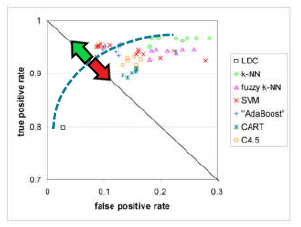
\includegraphics[width=3in]{Images/ROC} 
					\end{center}
				\end{minipage}
				%
				\paragraph{Precision/Recall} Mesures connues pour désigner la qualité d'un modèle. La \hl{précision} représente la 
					capacité à détecter seulement les occurrences pertinents ($\frac{TP}{TP + FP}$). Le \hl{rappel} représente
					le ratio de vrai positifs ($\frac{TP}{TP + FN}$).
				%
			%
		%
		\subsection{Optimiser classificateur}
			\begin{center}
				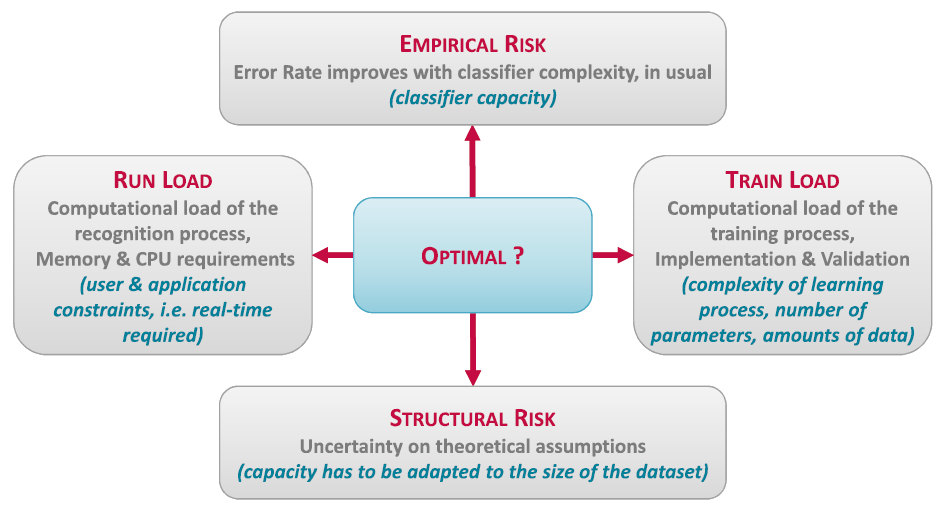
\includegraphics[width=6.75in]{Images/quality} 
			\end{center}
			%
			\alinea Améliorer le \hl{ratio de classifications correctes} d'un modèle représente une \hl{difficulté exponentielle}. 
				Passer de 50\% à 75\% de détection implique de diviser l'erreur par deux (50\% à 25\% d'erreur), et il faut aussi 
				diviser l'erreur par deux pour passer de 90\% à 95\% de détection (10\% à 5\% d'erreur).\\
			%
			~\\
			%
			\alinea Divers procédés existent pour améliorer la qualité d'un modèle. On peut essayer de générer d'autres données
				à partir de la base de données existante(\hl{Database boosting}). Le post-traitement permet d'améliorer la classification.
			%
		%
	%
	\section{Extraction d'attributs}
		\alinea Comme dit précédemment, cette étape peut se diviser en deux parties : l'extraction et la sélection des données.
		%
		\subsection{Extraction}
			\alinea Cette étape consiste à t\hl{raiter, filtrer et/ou nettoyer} les données brutes. Pour que cette étape soit réussie,
				il faut que les attributs extraits soient \red{discriminants}, c'est-à-dire qu'ils permettent d'avoir une 
				\hl{grande distance inter-classe et une petite distance intra-classe} dans les échantillons libellés.\\
			%
			\alinea Attention aux contraintes particulières comme la charge d'extraction, ou encore la compréhensibilité des attributs.
			%
		%	
		\subsection{Sélection}
			\alinea Mieux vaut utiliser \hl{le moins de dimensions possible} dans les données. En effet, au plus on a de dimensions, 
				au plus les chances de récolter des données avec autant de dimensions est faible, de plus, la discrimination peut être
				affaiblie par le nombre de dimensions. Cette étape consiste donc à réduire les dimensions utilisées par le modèle
				en filtrant les données inutiles, redondantes (permet alors de réduire le risque d'over-fitting) et/ou de faible qualité.
			%
		%
		\subsection{Clustering (Non-supervisé)}
			\alinea Traitement consistant à diviser l'ensemble de données en K clusters, avec K représentants appelés
				\hl{\textit{centroids}}.
			%
			\subsubsection{K-Means}
				\alinea Aussi appelé "E-M", K-Means consiste en un processus itératif visant à augmenter la distance inter-clusters
					et à minimiser la distance intra-clusters. On choisit des centroids (initialisation), puis on met à jour 
					l'appartenance de chaque données (\hl{expectation}) et enfin, on recalcule le centre de gravité du cluster qui sera
					le nouveau centroid du cluster (\hl{maximisation}). Les deux dernières étapes se répètent jusqu'à ce que les clusters
					ne varient plus de manière significative (selon un certain critère listé en bas à droite).
				%
				\begin{center}
					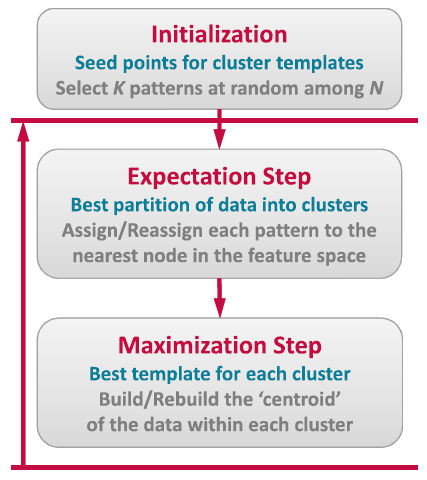
\includegraphics[width=2.5in]{Images/kmeans} 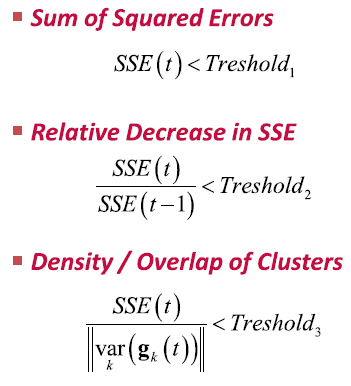
\includegraphics[width=2.5in]{Images/kmeans2} 
				\end{center}
				%
			%
			\subsubsection{Vector Quantization}
				\alinea Si la corrélation est prise en compte (en plus de la distance), le clustering peut alors servir de \hl{quantisation
					vectorielle}. C'est ce que fait le K-Means par défaut étant donné que les centroids sont des centres de gravité des 
					clusters.\\
				%
				~\\
				%
				\alinea Cette technique représente une alternative à la quantization scalaire qui veut que l'on prenne des 
					moyennes générales pour représenter les données. On prend alors le risque de se retrouver avec des clusters qui
					ne représentent aucune donnée.
				%
				\begin{center}
					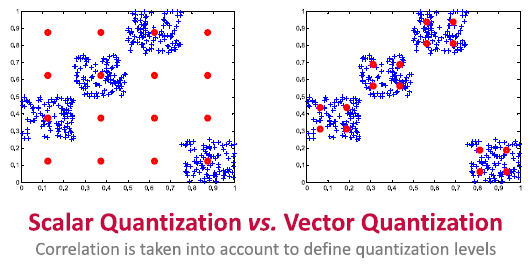
\includegraphics[width=3in]{Images/vector-quantization}
				\end{center}
				%
			%
			\subsubsection{Hierarchical clustering}
				\alinea Processus itératif visant à augmenter le nombre de clusters à chaque itération. L'\hl{avantage} de cette technique
					est que l'on ne doit pas fixer un nombre de cluster, et que l'on peut expérimenter plusieurs valeurs pour "K".
					Une manière de procéder est la \hl{duplication de centroid}. Par exemple, si on a 2 centroids, on les modifie
					avec du bruit, et on ré-effectue le clustering sur les 4 centroids obtenus de cette manière.	
				%
			%
		%
		\subsection{Analyse des composantes principales (PCA) (Non-supervisé)}
			\alinea Le principe de cette technique est de combiner les données existantes pour réduire le nombre de dimensions.
			%
			\subsubsection{KLT}
				\alinea Méthode permettant de trouver automatiquement des combinaisons entre les composantes.
				%
				\begin{center}
					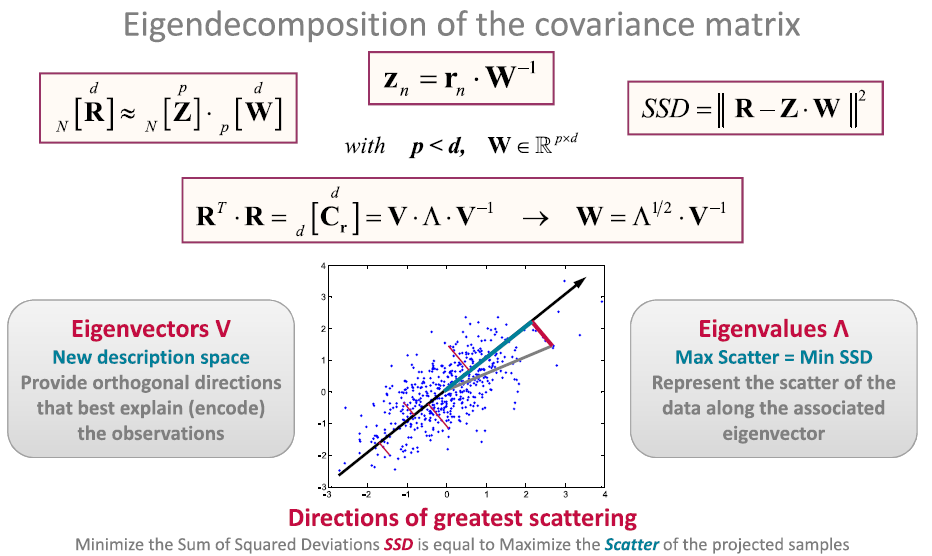
\includegraphics[width=5.5in]{Images/eigen}
				\end{center}
				%
				\alinea Les \hl{eigenvectors} sont à considérer comme de nouveaux axes à utiliser pour la classification. Les
					\hl{eigenvalues} permettent d'estimer la représentativité de l'eigenvector correspondant dans la classification 
					des données. Les vecteurs sont calculés grâce à la matrice de corrélation. En effet, la PCA vise à \hl{diagonaliser
					la matrice de corrélation des données}. Pour pouvoir appliquer une PCA, 
					il faut \hl{normaliser} les données en fonction de leur moyenne et de leur écart type 
					($y_n = \frac{r_n - \mu}{\sigma}$)	
				%
			%
			\subsubsection{PCA vs Clustering}
				\alinea La PCA est une \hl{alternative au clustering}. Effectuer les deux sur le même ensemble de données est inutile.
					\'Eventuellement, effectuer l'un puis l'autre permettrait de valider la première. 
					Les \hl{problèmes de la PCA} sont les suivants :
					\begin{itemize}
						\setlength\itemsep{0cm}
						\item Nouvelles dimensions peu compréhensibles car combinaisons d'anciennes dimensions.
						\item Le nombre de nouvelles dimensions à choisir est empirique car il est difficile de choisir le nombre
							idéal de dimensions permettant une classification optimale.
						\item Si les données ne sont pas normalisées, la PCA est inutile, ce qui implique que les dimensions
							perdent encore plus de leur signification (car sans unité, ...).
					\end{itemize}
				%
			%
			\subsubsection{Sélection des dimensions (Supervisé)}
				\begin{center}
					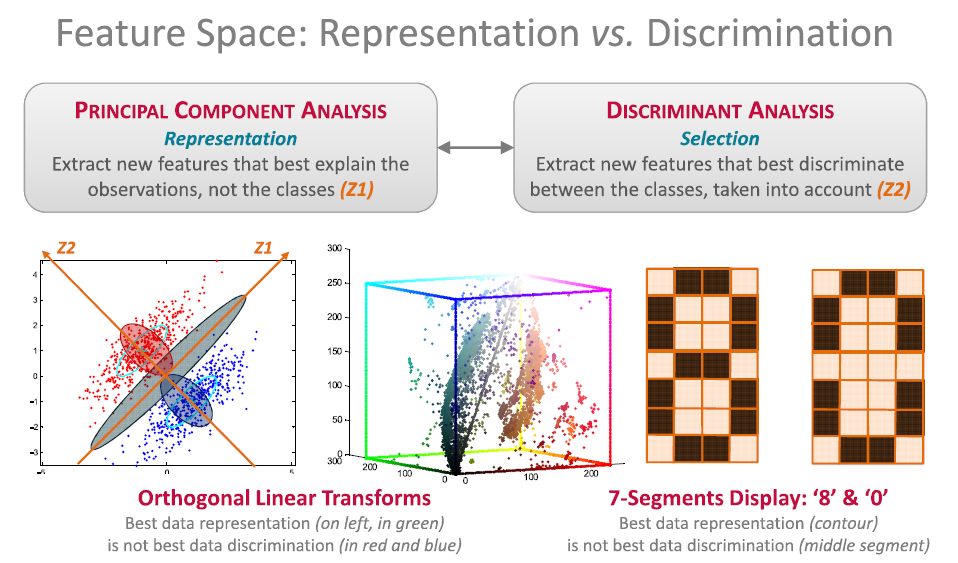
\includegraphics[width=\textwidth]{Images/pca}
				\end{center}
				%
				\paragraph{Méthodes wrapper} Entraîner le modèle en utilisant des sous-ensembles de nouvelles dimensions et choisir
					le modèle ayant la meilleure validation. \hl{Demande énormément de temps}.
				%
				\paragraph{Méthodes filtres} Calculer le score de chaque nouvelle dimension individuellement. Ce score ne permet pas de
					comparer plusieurs classifiers
					%
					\subparagraph{Discriminant de \hl{Fischer}} On attribue un score individuellement à chaque dimension en supposant 
						(risque	structurel) que les deux classes suivent une \hl{distribution gaussienne}. 
						$\Delta = \frac{(\mu_1 - \mu_2)^2}{\sigma_1^2 + \sigma_2^2}$. $\Delta = 6$ est un bon score pour une 
						distribution uniforme et $\Delta = 10$ est un bon score pour une distribution gaussienne.
					\subparagraph{Fischer généralisé} Méthode précédente adaptées aux cas impliquant plus que deux classes.
						Le calcul du discriminant est alors le suivant : 
						\hl{$\Delta = \frac{\text{Variance des moyennes}}{\text{Moyenne des variances}}$}.
					\subparagraph{Analyse de discriminant linéaire} Le principe est de remplacer la PCA suivie de la sélection de 
						dimension par une seule méthode. On se limite alors à $nb\_classes-1$ dimensions. C'est une mauvaise 
						technique si on a peu de classes (e.g. 2...).
				%
			%
		%
	%
%
\part{Classification}
	\alinea On peut distinguer deux types principaux de classificateurs : les classificateurs à correspondance de modèles 
		(\hl{pattern matching}), dont le temps d'\hl{exécution} peut être long, et les classificateurs \hl{paramétriques} qui sont 
		en général \hl{long à entraîner}.
	%
	\section{Probabilités de classe}
		\alinea Le but d'un classificateur est de réduire la probabilité d'erreur de classification. En reprenant plus haut la 
			définition du coût de classification erronée, on peut définir le risque de classification erronée, qui est probabiliste.
			$$ Risk(x) = 1 - P(\omega_i|x) $$
			On utilise ici la probabilité de classe \hl{à posteriori} ($P(\omega_i|x)$). Normalement, cette probabilité est difficile à
			calculer, mais le calcul est facilité par la loi de Bayes.
		%	
		\subsection{Probabilité à priori ($P(\omega_i)$)}
			\alinea La probabilité à priori représente la \hl{probabilité d'occurrence} d'une classe \hl{en règle générale}, sans 
				observation. Par exemple $P(femme)$ = 0.56 parce qu'il y a 56\% (random \%) de femmes sur Terre.
		%
		\subsection{Likelihood ($p(x|\omega_i)$)}
			\alinea Le likelihood (vraisemblance?) représente la probabilité de retrouver une observation $x$ dans la classe $\omega_i$.
				Ceci se fait aisément sur une base de données libellée, car il suffit de compter le nombre de données appartenant à la
				classe $\omega_i$ et répondant à l'observation $x$. Une observation est une caractéristique dimensionnelle. Par exemple
				$IR=255$ pour une image infrarouge.
		%
		\subsection{Fonction de densité ($p(x)$)}
			\alinea Probabilité en général de l'observation. En pratique, on peut la supprimer car on va comparer des probabilités de
				classes pour une observation fixe (faire varier $i$ de $\omega_i$, avec $x$ constante). 
				$$p(x) = \sum\limits^{i=1}_{m} p(x|\omega_i) \cdot P(\omega_i)$$
			%
		%
		\subsection{Probabilité à posteriori ($P(\omega_i|x)$)}
			\alinea Probabilité d'un vecteur de donnée d'appartenir à une classe $\omega_i$ en sachant que vecteur contient 
				l'observation $x$. Calculée en pratique grâce à la loi de Bayes. \hl{Les probabilités à posteriori sont discriminantes}
				dans un classificateur.
			%
		%
		
		\subsection{\hl{Loi de Bayes}}
			$$P(\omega_i|x) = \frac{P(\omega_i) \cdot p(x|\omega_i)}{p(x)}$$
			\alinea Les classificateurs Bayesien ont comme but de maximiser la probabilité a posteriori pour les données d'entraînement.
				$$ x \in \omega_i \Longleftrightarrow p(x|\omega_i) \cdot P(\omega_i)  >  p(x|\omega_j) \cdot P(\omega_j) $$
			%
		%
	%
	\section{Pattern matching}
		\subsection{k-Nearest Neighbours}
			\alinea L'idée est très simple : chercher dans le dataset les $k$ voisins les plus proches de la nouvelle donnée à classer,
				et libeller celle-ci selon la classe représentée \hl{majoritairement} dans ces $k$ voisins.
			%
		%
		\subsection{Clustering + kNN}
			\alinea L'idée est la même, mais pour réduire le temps de calcul, on va effectuer un clustering sur les données.
				Les k plus proches voisins ne seront alors plus des données de la base de données mais des \hl{centroids} de clusters.
				Il faut \hl{libeller chaque centroid}, car c'est les labels de ceux-ci qui seront comptés dans la procédure kNN.
		%
	%
	\section{Modèles paramétriques}
		\alinea Le principe ici est de construire un modèle qui va estimer la densité de probabilité des données et stocker les
			paramètres de ce modèle afin d'accélérer les calculs lors de la classification. La charge de calcul se trouve alors
			principalement dans l'entraînement.
		%
		\subsection{Modèles Gaussiens}
			\subsubsection{Modèle Gaussien naïf}
				\alinea Dans ce modèle, on va chercher $m \cdot d$ gaussiennes, c'est à dire \hl{une par dimension et par classe}.
					Pour chaque gaussienne, on va chercher sa \hl{moyenne et sa variance}.
				%
			%
			\subsubsection{Classificateur par distance Euclidienne}
				\alinea Même principe que le modèle précédent, mais on considère les variances et les probabilités à priori comme 
					étant égales pour toutes les classes.
				%
			%
			\subsubsection{Modèle à mélange de Gaussienne (GMM)}
				\alinea \'Etant donné que les modèles précédents avaient une capacité très faible et un risque structurel élevé (dû
					à la supposition que chaque classe suivait une distribution gaussienne), un nouveau modèle est né.
					Celui-ci suppose que l'on peut approximer la distribution de chaque classe par un \hl{mélange de plusieurs gaussiennes}.
					L'algorithme d'entraînement suit la logique du 'E-M':
					\begin{itemize}
						\setlength\itemsep{0cm}
						\item Expectation -- Estimer les probabilités des gaussiennes ($p(x|\theta)$)
						\item Maximisation -- Estimer les paramètres depuis les données ($p(\theta|x)$)
					\end{itemize}
				%
				\alinea Les GMM posent un risque structurel dû au \hl{choix du nombre de gaussiennes} par classe (risque d'over 
					ou d'underfitting). En effet, on ne peut pas ajouter autant de gaussienne que l'on veut car le nombre de données
					est fini. De plus, elles ont besoin d'un \hl{très grand nombre de données} pour obtenir un résultat précis.
				%
			%
		%
		\pagebreak
		%
		\subsection{Réseaux de neurones}
			\alinea Les réseaux de neurones sont des structures visant à simuler le fonctionnement du cerveau humain pour prendre
				des décisions. 
			%
			\subsubsection{Perceptron}
				\alinea Le plus simple modèle possible est celui définissant un unique neurone : le perceptron binaire.
					\begin{center}
						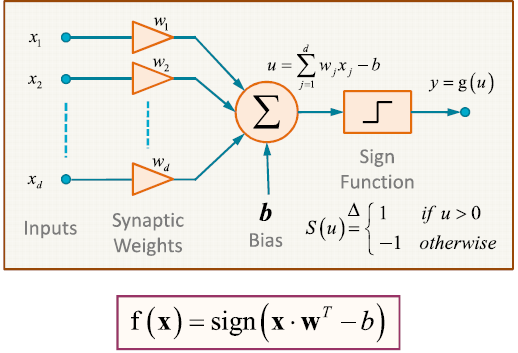
\includegraphics[width=3.75in]{Images/neuron}
					\end{center}
				%
				\alinea Ainsi que sa variante multi-classes : 
					\begin{center}
						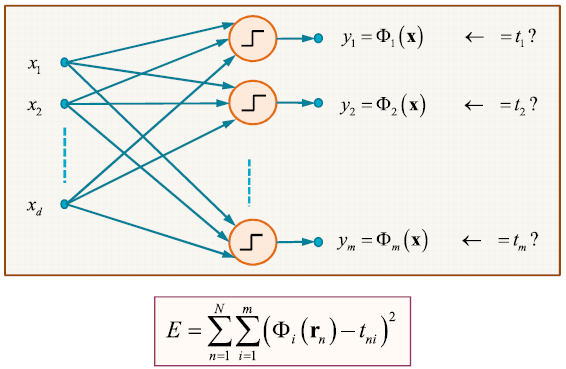
\includegraphics[width=3.75in]{Images/neuron2}
					\end{center}
				%
					Pour l'entraîner, il faut \hl{minimiser l'erreur} entre les label ($t_i$) et les résultats du modèle ($\Phi_i$).\\
				%
				~\\
				%
				\alinea Bien que \hl{linéaire}, l'entraînement permet de forcer la \hl{discrimination} entre les classes car les paramètres
					vont être entrainés afin d'essayer de renvoyer la bonne valeur pour chaque label, et ce en \hl{sélectionnant et en
					combinant automatiquement les dimensions utiles}.
				%
			%
			\subsubsection{Perceptron multi-couche (MLP)}
				\alinea Ce nouveau modèle permet d'obtenir une frontière de décision \hl{non-linéaire} de par la combinaison de fonctions
					d'activation non-linéaires. Il est prouvé que l'on peut approximer n'importe quelle fonction avec ce modèle,
					juste avec une couche cachée. Il faut alors faire varier les autres paramètres comme le nombre de neurones et 
					les fonctions d'activation pour arriver à approximer la fonction voulue. Lorsqu'on empile les couches, l'effet
					\hl{boite noire} est de mise pour les réseaux de neurones. En effet, leur intérieur devient très complexe à 
					comprendre et à déboguer.\\
				%
				~\\
				%
				\alinea Les fonctions d'activations doivent respecter certaines \hl{conditions} : 
					\begin{itemize}
						\setlength\itemsep{0cm}
						\item Être non-linéaires -- elles seraient inutiles sinon
						\item Être continues et dérivables
						\item Approximer une décision binaire dans le cas d'un classificateur
					\end{itemize}
				%
				\begin{center}
					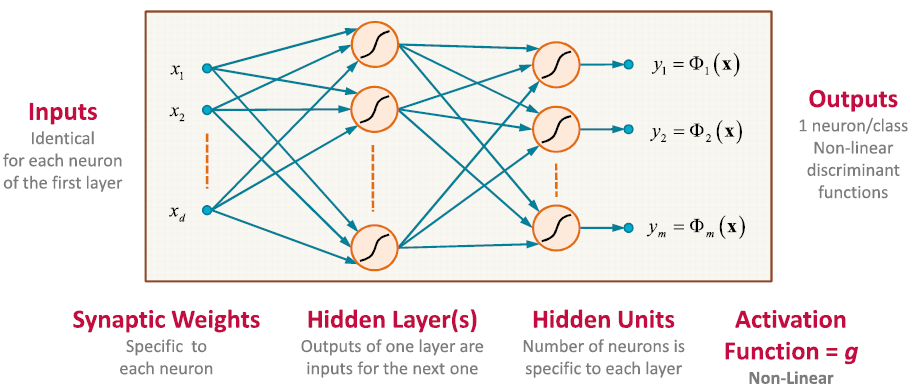
\includegraphics[width=6in]{Images/mlp}
				\end{center}
				%
				\alinea La sortie d'un MLP représente la probabilité d'appartenir à une certaine classe. Ces probabilités sont une 
					\hl{approximation des probabilités à posteriori}. Il y a une sortie par classe, et les labels valent 1 (appartient)
					ou 0 (n'appartient pas). \'Etant donné que ces probabilités sont des probabilités a posteriori, on peut jouer
					sur la formule vu précédemment. \red{Dans le cas ou la probabilité à priori change}, on doit juste diviser
					la sortie du réseau par l'ancienne probabilité et la multiplier par la nouvelle probabilité. \\
				%
				~\\
				%
				\alinea Dans le cas où un MLP n'arrive pas à classifier certaines instances de données, on peut 
					\hl{combiner plusieurs MLPs}
					pour obtenir de meilleurs résultats. On peut par exemple entraîner un MLP spécialisé dans les instances que
					le premier MLP a du mal à classer. Ou encore, proposer plusieurs MLPs et faire appels aux plus gros et couteux en
					temps qu'en cas de besoin.
				%
			%
			\subsubsection{Entraînement}
				\alinea Basé sur une règle de "\hl{Least Squared Error}" (mise à jour itérative des poids synaptiques).
					La méthode utilisée pour optimiser les poids est la \hl{descente de gradient}. Elle est très lourde,
					mais efficace. Pour s'entraîner, un réseau va faire appel à un algorithme de \hl{Backpropagation} :
					\begin{enumerate}
						\setlength\itemsep{0cm}
						\item Initialisation -- Valeurs aléatoires pour les poids.
						\item Pour chaque donnée d'entraînement:	
							\begin{enumerate}
								\setlength\itemsep{0cm}
								\item Calculer les gradients en fonction de la sortie et du label attendu.
								\item Mettre à jour les poids en fonction des gradients calculés.
							\end{enumerate}
						\item Répéter l'étape précédente jusqu'à ce que l'évolution des poids ne soit plus 'significative'.
					\end{enumerate}
					On peut éventuellement accélérer le processus en \hl{pré-traitant} les données d'entraînement (réduire la dimensionalité
					ou entraîner sur des centroids de clusters).
				%
				\paragraph{Entraînement On-line vs. Batch} 
					\begin{itemize}
						\setlength\itemsep{0cm}
						\item On-line -- A chaque donnée présentée, les poids sont mis à jour. \hl{Plus rapide} pour converger, 
							mais \hl{moins bonne approximatio}n de l'erreur globale.
						\item Batch -- On met à jour les poids qu'après la présentation de toute la base de données. \hl{Plus lent} 
							à converger mais \hl{meilleure approximation} de l'erreur globale.
					\end{itemize}
					Un bon compromis entre les deux est un \hl{entraînement par petits batchs} (une fraction de la base de données 
					est présentée, on met à jour les poids, puis on recommence...).
				%
				\paragraph{Momentum term} \'Evolution douce des gradients afin d'être \hl{moins sensible au bruit}.
					Les poids de l'instant $\tau - 1$ sont ajoutés dans le calcul des poids ) l'instant $\tau$. On doit choisir
					deux paramètres : $\alpha$ et $\beta$. Ceux-ci doivent être choisi au cas par cas afin d'éviter les minima locaux
					dans les calculs.
				%
				\paragraph{Variable Learning Rate (Vogl)} Méthode \hl{très rapide (dans les cas des MLP à une couche cachée)} 
					se basant sur la méthode précédente, mais où $\beta$ n'est pas nécessaire et où \hl{$\alpha$ est adaptatif}. 
				%
				\paragraph{Diagonal Levenberg-Marquadt (DLM)} Approximation d'une \hl{minimisation du second ordre}. Le principe est de 
					calculée une matrice hessienne (minimisation du second degré) sur un petit groupe de données (K données) et de ne 
					\hl{garder que les éléments de la diagonale} (risque structurel car suppose que les autres éléments sont inutiles). 
					On peut choisir \hl{K comme étant le nombre de classe} et\hl{ attendre d'avoir un représentant par classe} avant de 
					mettre à jour les poids. Cette méthode permet de mieux gérer un \hl{grand nombre de couches cachées}.
				%
				\paragraph{Minima local} ~\\~\\
					\begin{minipage}{0.8\textwidth}
						Les calculs de \hl{gradients locaux} avec une fonction sigmoid provoquent des \hl{minima locaux} 
						qui peuvent perturber l'entraînement. En effet, la sigmoid crée des termes "en chapeaux" et dés qu'on trouve 
						un zéro, le calcul de gradient s'arrête. Au plus il y a de couches cachées, au plus ce risque est grand. 
						\hl{Prendre des petits poids comme valeurs initiales} peuvent aider car on voudrait rester proche de 0.
						\hl{Utiliser la fonction "cross-entropy"} pour calculer l'erreur aide à réduire ce risque car on augmente 
						la dérivée des valeurs cibles (targets).
					\end{minipage}\hfill
					\begin{minipage}{0.19\textwidth}
						\begin{center}
							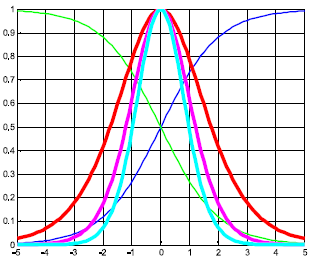
\includegraphics[width=1.5in]{Images/sigmoid}
						\end{center}			
					\end{minipage}
					%
				%
				\paragraph{Besoin de validation} Comme la capacité des réseaux de neurones est très grande, le risque d'overfitting est
						grand. 
						C'est pourquoi une \hl{validation de taille importante} est requise pour que l'algorithme puisse s'arrêter
						avant d'overfitter.
					%
				%
			%
			\subsubsection{Réseaux complexes}
				\paragraph{Self-Organizing Maps (SOM)} Ces réseaux font un \hl{clustering} (entraînement non-supervisé) \hl{spatial}. 
						Leur entraînement se fait grâce à une mise à jour des poids en fonction des voisinages des clusters.
						Le principe est de considérer chaque \hl{neurone} comme étant le \hl{centroid} d'un cluster.
						Il suffit ensuite de sélectionner le \hl{label présent majoritairement} dans l'entourage de chaque neurone.\\
					%
					~\\
					%
					\alinea Ils produisent des frontières de décision \hl{linéaires par morceau}. En pratique, les SOM sont utilisés
						pour \hl{mieux comprendre des données à haute dimensionalité}. On peut améliorer leur résultats 
						en appliquant un post-entraînement "LVQ" (Learning Vector Quantization) qui permet de réduire la distances
						intra-clusters et d'augmenter la distance inter-cluster en utilisant les labels (entraînement supervisé).
					%
					\begin{center}
						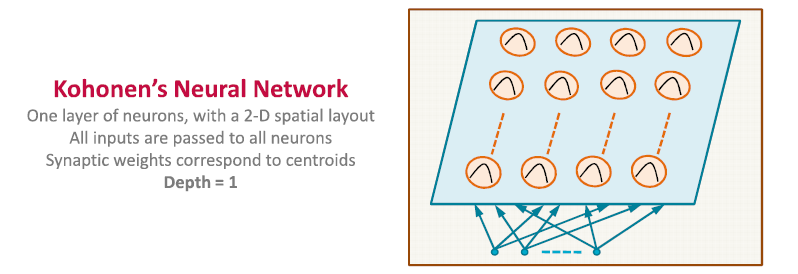
\includegraphics[width=6.5in]{Images/som}
					\end{center}
					%
				%
				\paragraph{Radial Basis Function (RBF)} ~\\~\\
					\begin{minipage}{0.65\textwidth}
						MLP à une couche cachée. Le rôle de cette dernière est d'\hl{estimer la
					densité de probabilité représentant les centroids résultats d'un clustering} (également fait par la couche cachée). 
					Ces modèles sont \hl{plus faciles à entraîner} qu'un MLP classique mais \hl{non-optimal}. De plus, le \hl{runtime}
					de ceux-ci sont \hl{plus élevés} car ils ont besoin de plus de neurones qu'un MLP classique.
					\end{minipage}\hfill
					\begin{minipage}{0.33\textwidth}
						\begin{center}
							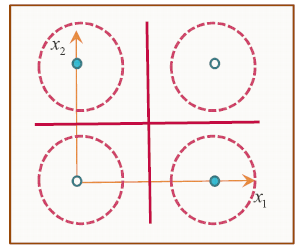
\includegraphics[width=2.5in]{Images/rbf}
						\end{center}			
					\end{minipage} 
				%
				\paragraph{Précautions pour réseaux profonds}
					\alinea Vu que les réseaux profonds sont des modèles très complexes, \hl{plusieurs précautions sont à prendre}
						afin de limiter le risque structurel..
						\begin{center}
							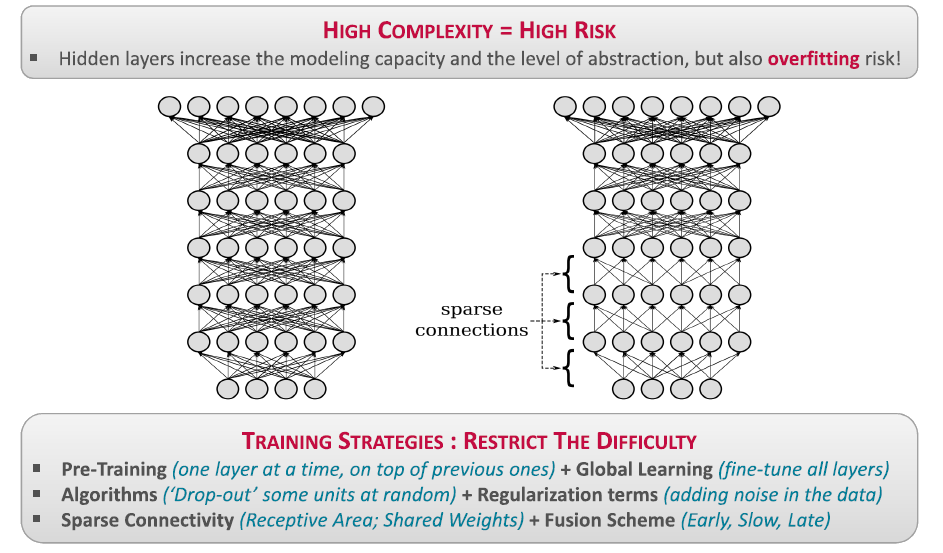
\includegraphics[width=\textwidth]{Images/deep}
						\end{center}
						\begin{center}
							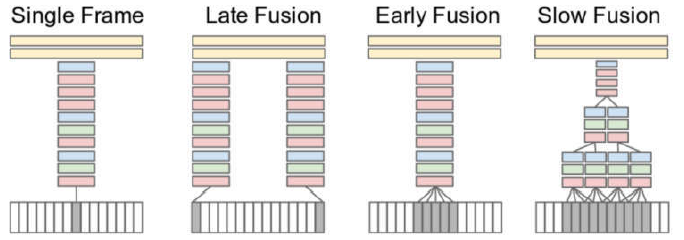
\includegraphics[width=0.75\textwidth]{Images/fusion}
						\end{center}
					%
				%
				\pagebreak
				%
				\paragraph{Réseaux convolutionnels (auto-encoders)}
					\alinea Ces réseaux ont la particularité d'\hl{extraire eux-même des attributs} intéressants depuis les 
						\hl{données brutes}. L'avantage est que \hl{l'entraînement de ce réseau est discriminant} car on vise une 
						optimisation globale (on chercher à correspondre aux labels targets). L'algorithme d'entraînement 
						utilisé est \hl{DLM}.
						\begin{center}
							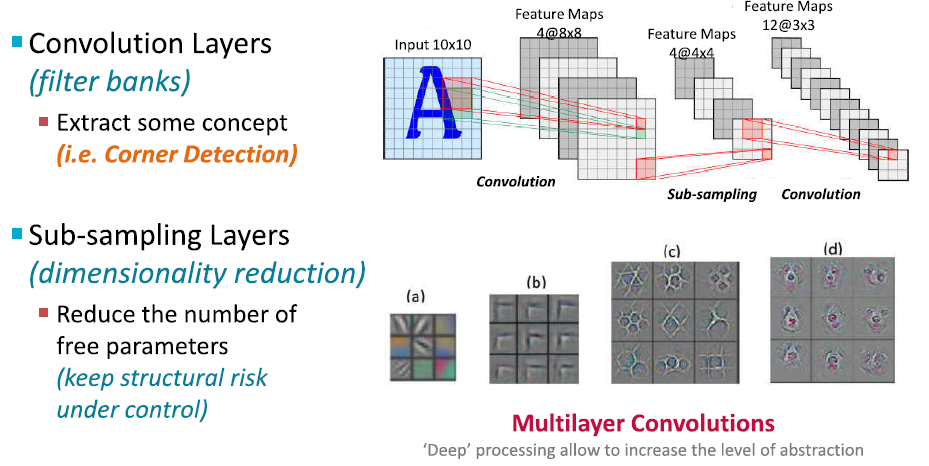
\includegraphics[width=\textwidth]{Images/cnn}
						\end{center}
					%
					\alinea Un \hl{MLP est généralement placé en sortie} de ce réseau d'extraction d'attribut pour jouer le rôle de
						classificateur sur les attributs fraîchement extraits. 
					%
				%
			%
		%	
		\subsection{Support Vector Machines (SVM)}
			\alinea le principe ici est d'établir une frontière linéaire entre deux classes, et de maximiser la marge existant entre les
				représentants de chaque classe. Ceci revient donc à maximiser $\frac{2}{\|w\|}$ et donc à \hl{minimiser $J = \|w\|^2$}.
				Les support vectors à proprement parler sont \hl{P1 et P2}. Ce seront les \hl{seuls représentants du modèle} après
				l'entraînement.
				\begin{center}
					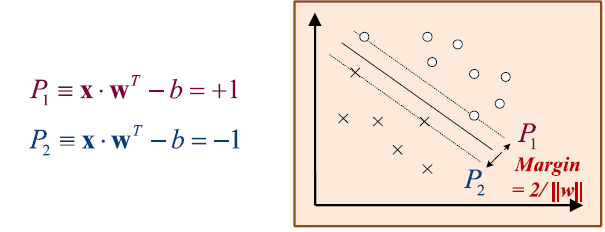
\includegraphics[width=3in]{Images/svm}
				\end{center}
			%
			\subsubsection{Entraînement}
				\alinea L'entraînement est un problème quadratique. Le but est de maximiser la marge sous la contrainte qu'\hl{aucune
					donnée ne peut se situer entre P1 et P2}. On peut définir les \red{support vectors} comme étant des points qui \hl{ne
					peuvent être retirés} sans modifier la frontière de décision. \\
				%
				~\\
				%
				\begin{minipage}{0.65\textwidth}
					\alinea Lorsque des données ne sont pas séparables sont cette contrainte (bruit ou frontière impossible), il 
						faut alors définir une constante de pénalité $C$ qui représente le coût d'erreur de classification. Le but
						sera alors de \hl{maximiser la marge en minimisant le coût induit par $C$}. Si $C$ est petit, la marge sera
						grande, on parle alors \hl{d'undertraining}, tandis que si sa valeur est élevée, la marge sera toute petite,
						diminuant les erreurs d'entraînement, mais réduisant la claire séparation entre les classes, on parle alors
						d'\hl{overtraining}.
				\end{minipage}\hfill
				\begin{minipage}{0.33\textwidth}
					\begin{center}
						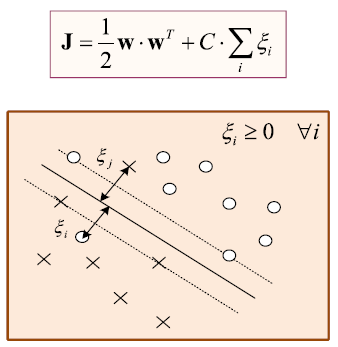
\includegraphics[width=2in]{Images/svm2}
					\end{center}			
				\end{minipage} ~\\~\\~\\
				%
			%
			\subsubsection{classification non-linéaire}
				\alinea Pour classer de manière non-linéaire, on va \hl{augmenter le nombre de dimension} de nos données en fournissant
					un \hl{mapping non-linéaire}. On aura alors une frontière linéaire dans l'espace augmenté et une classification 
					non-linéaire dans l'espace de base.
				\begin{center}
					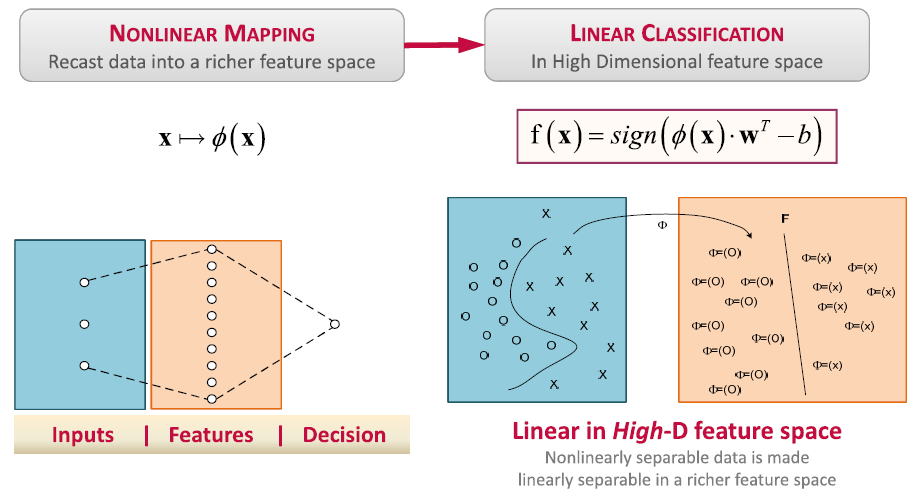
\includegraphics[width=0.66\textwidth]{Images/svm3}
				\end{center}
				%
				\alinea Pour optimiser les calculs, on passe généralement par une "\hl{fonction Kernel}" remplaçant le produit scalaire
					entre vecteurs de très hautes dimensionalité (espace augmenté). Cette fonction dépend du mapping entre l'espace
					initial et l'espace augmenté et \hl{permet d'effectuer les calculs sur les dimensions initiales.}
				%
				\begin{center}
					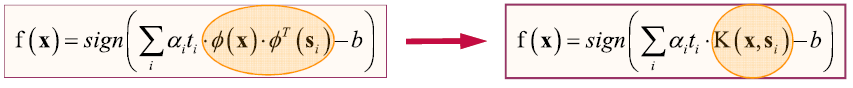
\includegraphics[width=0.66\textwidth]{Images/svm4}
				\end{center}
				%
				\alinea Plusieurs types de kernels sont donnés dans l'image suivante:
					\begin{center}
						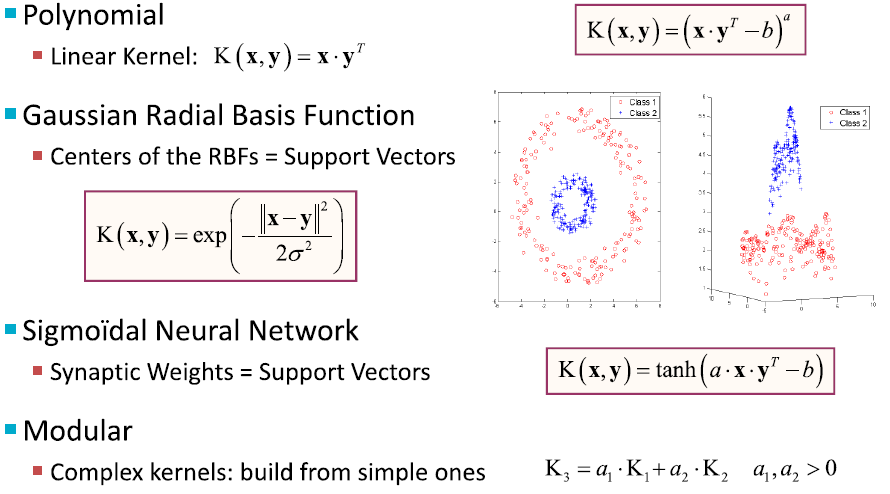
\includegraphics[width=0.66\textwidth]{Images/kernels}
					\end{center}
				%
				\alinea Comme on cherche des support vectors, et plus une liste de likelihood de toutes les données (Réseaux de neurones),
					le processus d'entraînement est plus rapide. On peut noter que \hl{les dimensions intrinsèques} aux données 
					\hl{restent les même dans l'espace augmenté}. \hl{On contrôle le risque structurel par le nombre de dimensions
					choisi.} De plus, en prenant le \hl{bon kernel}, le risque d'overfitting si on prend \hl{plus de dimensions que
					nécessaire} est faible. \hl{Les SVMs sont donc plus rapides à entraîner que les réseaux de neurones mais leur
					temps de calcul pour classer est bien supérieur ! (La qualité du résultat est similaire). Les SVM demandent
					moins de données que les réseaux de neurones pour être efficaces.}
				%
			%
			\subsubsection{Problème multi-classes}
				\alinea \hl{Les SVMs sont fait pour séparer de manière binaire}. Pour des problèmes multi-classes, des stratégies 
					particulières doivent être adoptées : 
					\begin{itemize}
						\setlength\itemsep{0cm}
						\item One-Against-All (\hl{OvA}) -- Une SVM par classe (appartient à classe m ou appartient à une autre classe).
						\item One-Against-One (\hl{OvO}) -- Une SVM par paire de classes. On sélectionne alors par un vote majoritaire.
					\end{itemize}
					Dans tous les cas, on n'obtiendra pas des probabilités à posteriori en sortie.
				%
			%
			\subsubsection{Grandes bases de données}
				\alinea Afin de réduire les calculs, on entraîne plusieurs SVMs sur des \hl{sous-ensembles de données}. On les combine 
					ensuite en \hl{gardant uniquement les support vectors}.
				%
			%
			\subsubsection{Utilités diverses des kernels}
				\begin{center}
					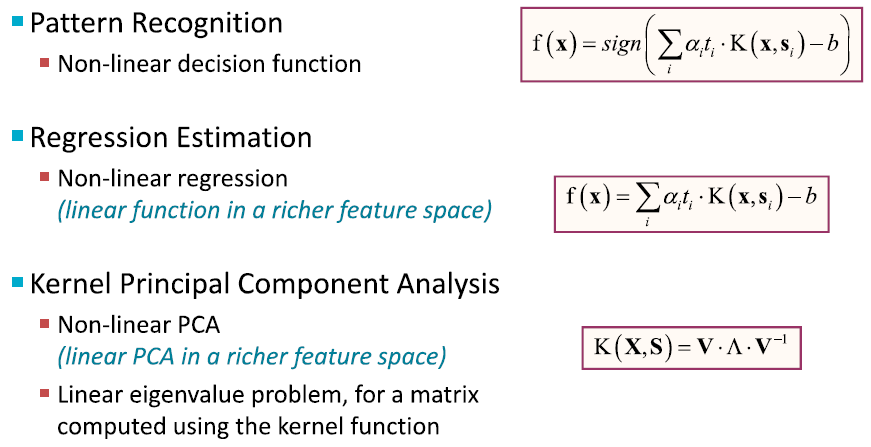
\includegraphics[width=0.66\textwidth]{Images/kernels2}
				\end{center}
				%
			%
		%			
	%
	\section{Comparer des classificateurs}
		\subsection{Combiner des classificateurs}
			\alinea Il existe plusieurs manières d'interpréter les sorties de plusieurs classificateurs. On peut faire la \hl{somme} des
				probabilités donnés par chaque classificateurs et prendre la somme majoritaire, on peut également faire le \hl{produit}
				(très sensibles aux petites valeurs), prendre les probabilités \hl{maximum} ou \hl{minimum}, prendre la probabilité 
				\hl{médiane} (celle qui se trouve à la foin le plus loin du max et le plus loin du min). On peut également
				faire un vote de majorité en fonction de la décision de chaque classificateur.
			%
		%
		\subsection{\\hl{'Evaluation des classificateurs}}
			\alinea De 5 (Excellent) à 1 (Faible) :
				\begin{center}
					\begin{tabular}{|l|c|c|c|c|}
						\hline
						\textbf{Technique} & \textbf{Risque empir.} & \textbf{Risque struct.} & \textbf{Temps entr.} & 
							\textbf{Temps exec.}\\
						\hline
						KNN & 5 & 5 & 5 & 1\\
						\hline
						KMeans & 3 & 3 & 3 & 3 \\
						\hline
						GMM & 4 & 2 & 2 & 3 \\
						\hline
						MLP & 5 & 2 & 1 & 4 \\
						\hline
						RBF & 5 & 2 & 2 & 3 \\
						\hline
						SVM & 5 & 3 & 3 & 2 \\
						\hline
					\end{tabular}
				\end{center}
			%
			\paragraph{KNN}
				\alinea Le temps d'exécution est long car ça prend du temps de chercher après les N plus proches voisins
				%
			%
			\paragraph{Kmeans}
				\alinea Est "moyen" partout car il est vraiment bon en rien, mais pas mauvais
					non plus. On a besoin de modéliser les données, donc le temps d'exécution est moyen également.
				%
			%
			\paragraph{GMM}
				\alinea Le risque empirique est présent car l'entraînement n'est pas discriminant. Le risque structurel est élevé car
					il faut choisir le nombre de gaussiennes. L'entraînement peut être long car itératif et beaucoup de paramètres.
					Le temps d'exécution est moyen car besoin de modéliser les données.
				%
			%
			\paragraph{MLP}
				\alinea Entraînement très long du au nombre de paramètres. Risque structurel élevé du à un choix important de paramètres
					(nombre de couches et neurones, ...).
				%
			%
			\paragraph{SVM}
				\alinea Apprentissage discriminant qui permet d'avoir peu de risque empirique. Temps d'exécution élevé, surtout 
					si multi-classes ! Le risque structurel vient de l'augmentation du nombre de dimensions pour une classification
					non-linéaire.
				%
			%
		%
	%
	\section{Systèmes dynamiques}
		\alinea Lorsque l'on veut classer des données ayant des dépendances temporelles, des modèles plus spécifiques doivent être
			utilisés.
		%
		\subsection{Dynamic Time Warping (DTW)}
			\alinea Le principe est de trouver un chemin faisant un \hl{mapping} entre deux séquences temporelles.
				Là où la méthode la plus simple serait de faire un mapping linéaire (NB les indices commencent à 1 dans l'image
				ci-dessous):
				\begin{center}
					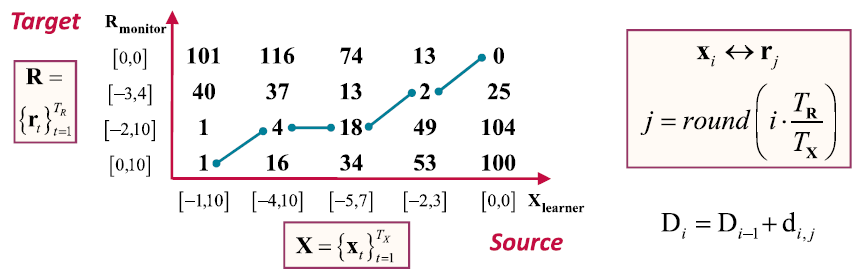
\includegraphics[width=0.75\textwidth]{Images/dtw1}
				\end{center}
			%
			Un mapping plus complexe va être recherché. Ce mapping doit respecter certaines \hl{contraintes} : 
				\begin{itemize}
					\setlength\itemsep{0cm}
					\item La causalité des données  -- \hl{ne pas revenir dans le temps} 
					\item La continuité et la symétrie entre les séquences -- aller \hl{au bout des séquences} et \hl{utiliser toutes les
						frames}
				\end{itemize} 
				Au final, on veut minimiser la distance globale du chemin à parcourir.
			%
			\begin{center}
				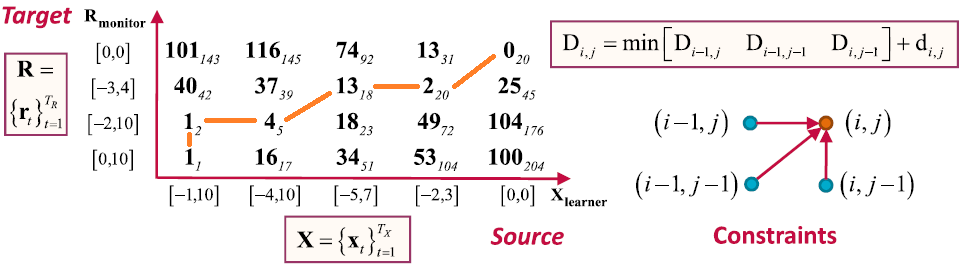
\includegraphics[width=0.9\textwidth]{Images/dtw2}
			\end{center}
			%
			\subsubsection{Weighted DTW}
				\alinea Cette variante promeut les \hl{chemins diagonaux} en pénalisant les accès verticaux et horizontaux.
					De plus, les \hl{$\lambda$ peuvent être ajustés afin d'intégrer des probabilités à priori}.
				%
				\begin{center}
					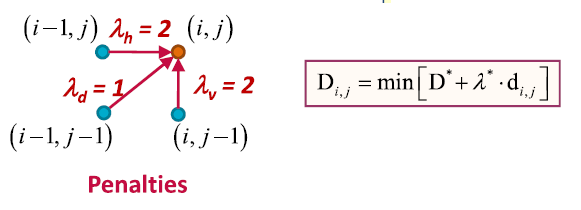
\includegraphics[width=0.5\textwidth]{Images/dtw3}
				\end{center}
				%
			%
			\subsubsection{DTW asymétrique}
				\alinea Des contraintes / relaxations supplémentaires peuvent être ajoutées au problèmes. En effet, on peut
					ajouter des chemins possibles (+3 chemins par étape) ou supprimer certains chemins.
					\begin{center}
						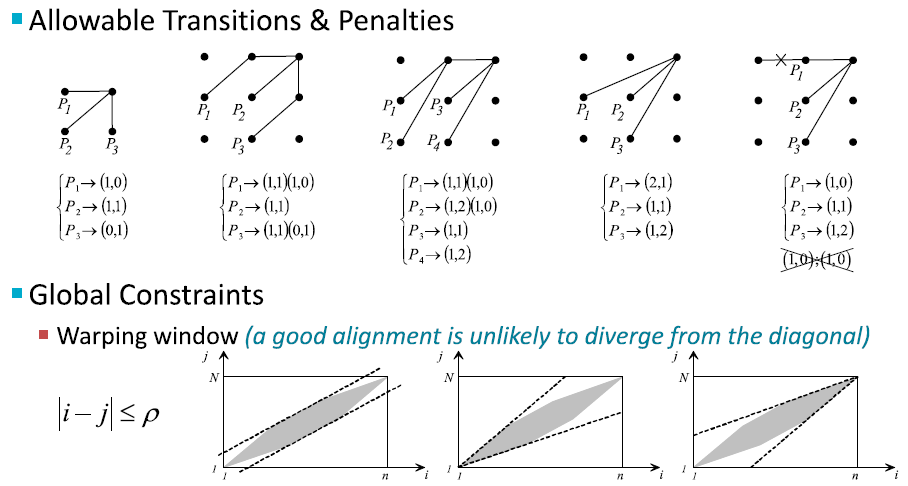
\includegraphics[width=0.9\textwidth]{Images/dtw4}
					\end{center}
				%
			%
			\subsubsection{Classification}
				\alinea Pour classifier en utilisant le DTW, on peut effectuer un clustering et \hl{comparer} les nouveaux
					vecteurs temporels \hl{avec les centroids}.
				%
			%
		%
		\subsection{Modèles de Markov}
			\alinea Les modèles de Markov sont des machines à états probabilistes qui ont deux types de probabilités : 
				celles de transitions et celles d'émission. Leur \hl{capacité doit être adaptée} à la complexité du problème
				(GMM, MLP, ... c.f. variantes).
				\begin{center}
					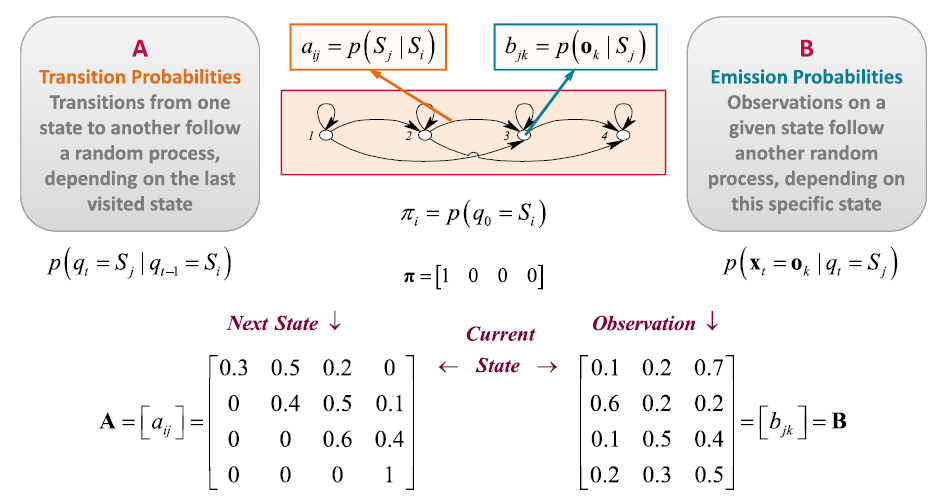
\includegraphics[width=0.9\textwidth]{Images/hmm}
				\end{center}
			%
			\begin{center}
				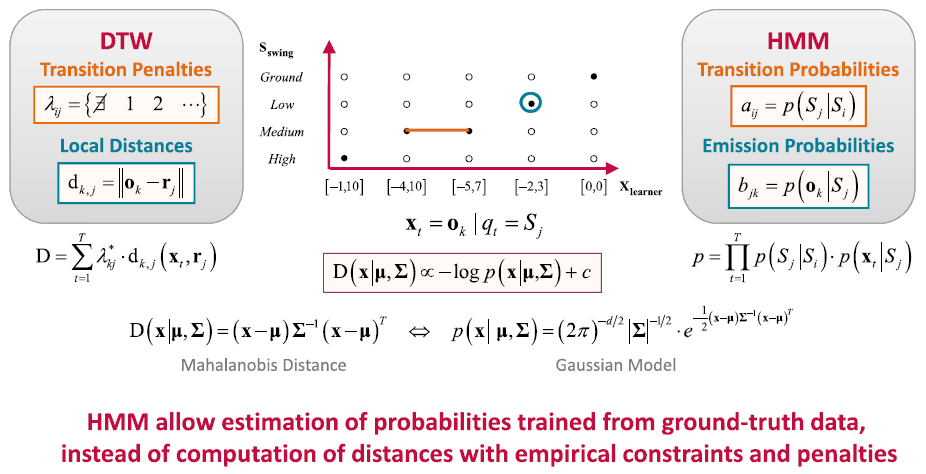
\includegraphics[width=0.9\textwidth]{Images/hmm2}
			\end{center}
			%
			\alinea Pour \hl{estimer la probabilité} d'une donnée, il suffit de faire la somme de tous les chemins possibles. 
				Pour \hl{estimer la succession d'état} la plus probable, il ne faut prendre en compte que le chemin le plus
				probable (décodage de Viterbi). Pour l'\hl{entraîner}, on suit l'algorithme de Viterbi : 
				\begin{itemize}
					\setlength\itemsep{0cm}
					\item Initialisation -- alignement linéaire des observations et des états.
					\item Expectation -- Estimation des probabilités de transitions et d'émission en comptant simplement
						les occurrences dans les données.
					\item Maximisation -- Améliorer l'alignement entre les observations et les états par décodage de Viterbi).
				\end{itemize}
				Note : En général, on utilise le logarithme des probabilités pour éviter de traiter ave des trop petits nombres 
				(multiplication de proba).	
			%
			\subsubsection{Variante à temps continu}
				\begin{minipage}{0.69\textwidth}
					\alinea Lorsqu'on ne peut pas diviser le temps en étape, on peut toujours assigner un GMM à chaque état du HMM.
						Il faut alors choisir le nombre de gaussienne par état. Exemple avec 4 états et 2 gaussiennes par état.
				\end{minipage}\hfill
				%
				\begin{minipage}{0.3\textwidth}
					\begin{center}
						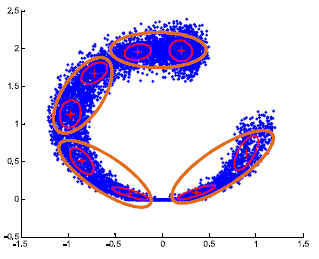
\includegraphics[width=1.5in]{Images/hmm3}
					\end{center}
				\end{minipage}
				%
			%
			\subsubsection{Variante hybride MLP}
				\alinea Pour estimer les probabilités à posteriori, on peut mélanger MLP et HMM. On obtient de très bons résultats
					mais le risque structurel explose et le temps d'entraînement aussi.	
				%
			%
		%
		\subsection{Comparaison (au plus = au mieux)}
			\begin{center}
				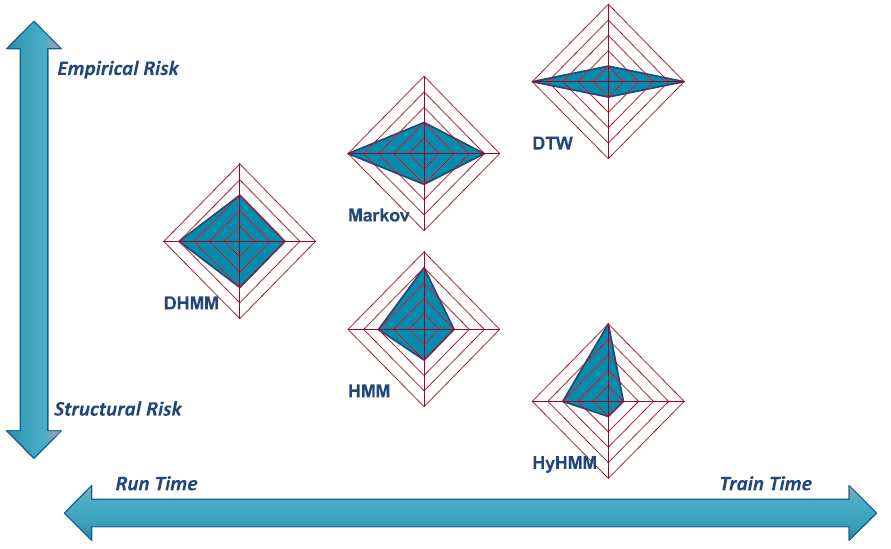
\includegraphics[width=0.7\textwidth]{Images/comp}
			\end{center}
		%
	%
%
\end{document}